One of the major achivements by the ATLAS and CMS collaborations during the Run1 data taking at a centre-of-mass energy of 8 TeV  at the Large Hadron Collider (LHC) is the discovery of a scalar particle, with a mass of approximately 125 GeV, and properties  consistent with the Higgs boson predicted in the Standard Model (SM). 
 An important question is whether this new particle is the SM Higgs boson or part of an extended Higgs sector. One interesting approach to answer this question is to search for additional scalars.
For the first LHC collision data provided at a centre-of-mass energy of 13 TeV and recorded
by the ATLAS and CMS detectors, the collaborations have performed many searches that are
motivated by a variety of models beyond the SM. The simplest extensions of the SM involve the
addition of a singlet or  the addition of a doublet field, known as Electroweak Singlet Models (EWS)
and Two-Higgs-Doublet Models (2HDM), respectively. Many searches are motivated by these
extensions and benchmarks within specific related models, such as the Minimal Supersymmetric
Standard Model (MSSM). The MSSM in a particular benchmark scenario is completely
determined by two parameters, the mass of one of the Higgs bosons and the ratio of the vacuum
expectation values, tan$\beta$. Models in which both both an additional singlet and doublet field are added in the Higgs sector have been proposed, and benchmarks in the Next to Minimal Supersymmetric
Standard Model (NMSSM) have motivated several additional searches at the LHC. Finally extension with triplets fields has been searched by both the ATLAS and the CMS collaborations.

In this proceeding will detail  on the new searches performed with the 13 TeV
data, which are performed with an integrated luminosity of 3.2 fb$^{-��1}$ and up to 2.3 fb$^{-1}$ with the
ATLAS \cite{ATLAS-CONF-2015-061,HH_bbbb_ATLAS,HH_bbgg_ATLAS,chargedH_tb_ATLAS,chargedH_tuanu_ATLAS} and CMS \cite{HH_bbtautau_CMS,HH_bbWW_CMS,HH_bbbb_CMS} detectors, respectively. In particular, we will focus on the searches of new scalar bosons in the MSSM benchmarks. Both the wide variety of searches and the precise measurement of the Higgs boson couplings  performed with an integrated luminosity of  20 fb$^{-1}$ at $\sqrt{s}=$8 TeV by the ATLAS \cite{aa3photon} and the CMS \cite{Hmumu_ref_CMS,Hbb_ref_CMS,chargedH_tb_CMS,diChargedH} collaborations put stringent limits on the MSSM parameter space. In figure \ref{fig:MSSM_Run1} is shown the Run1 results by ATLAS and CMS collaborations \cite{Aad2015,CMS-PAS-HIG-16-007}. Among the new searches performed with the 13 TeV data, the $A/H\rightarrow\tau\tau$ and the $H\rightarrow hh$ are particularly intriguing and already able to investigate regions of the MSSM parameter space not covered before. 
For this reason, this proceeding will focus on these two searches.

 %%
\begin{figure}[htb]
\centering
	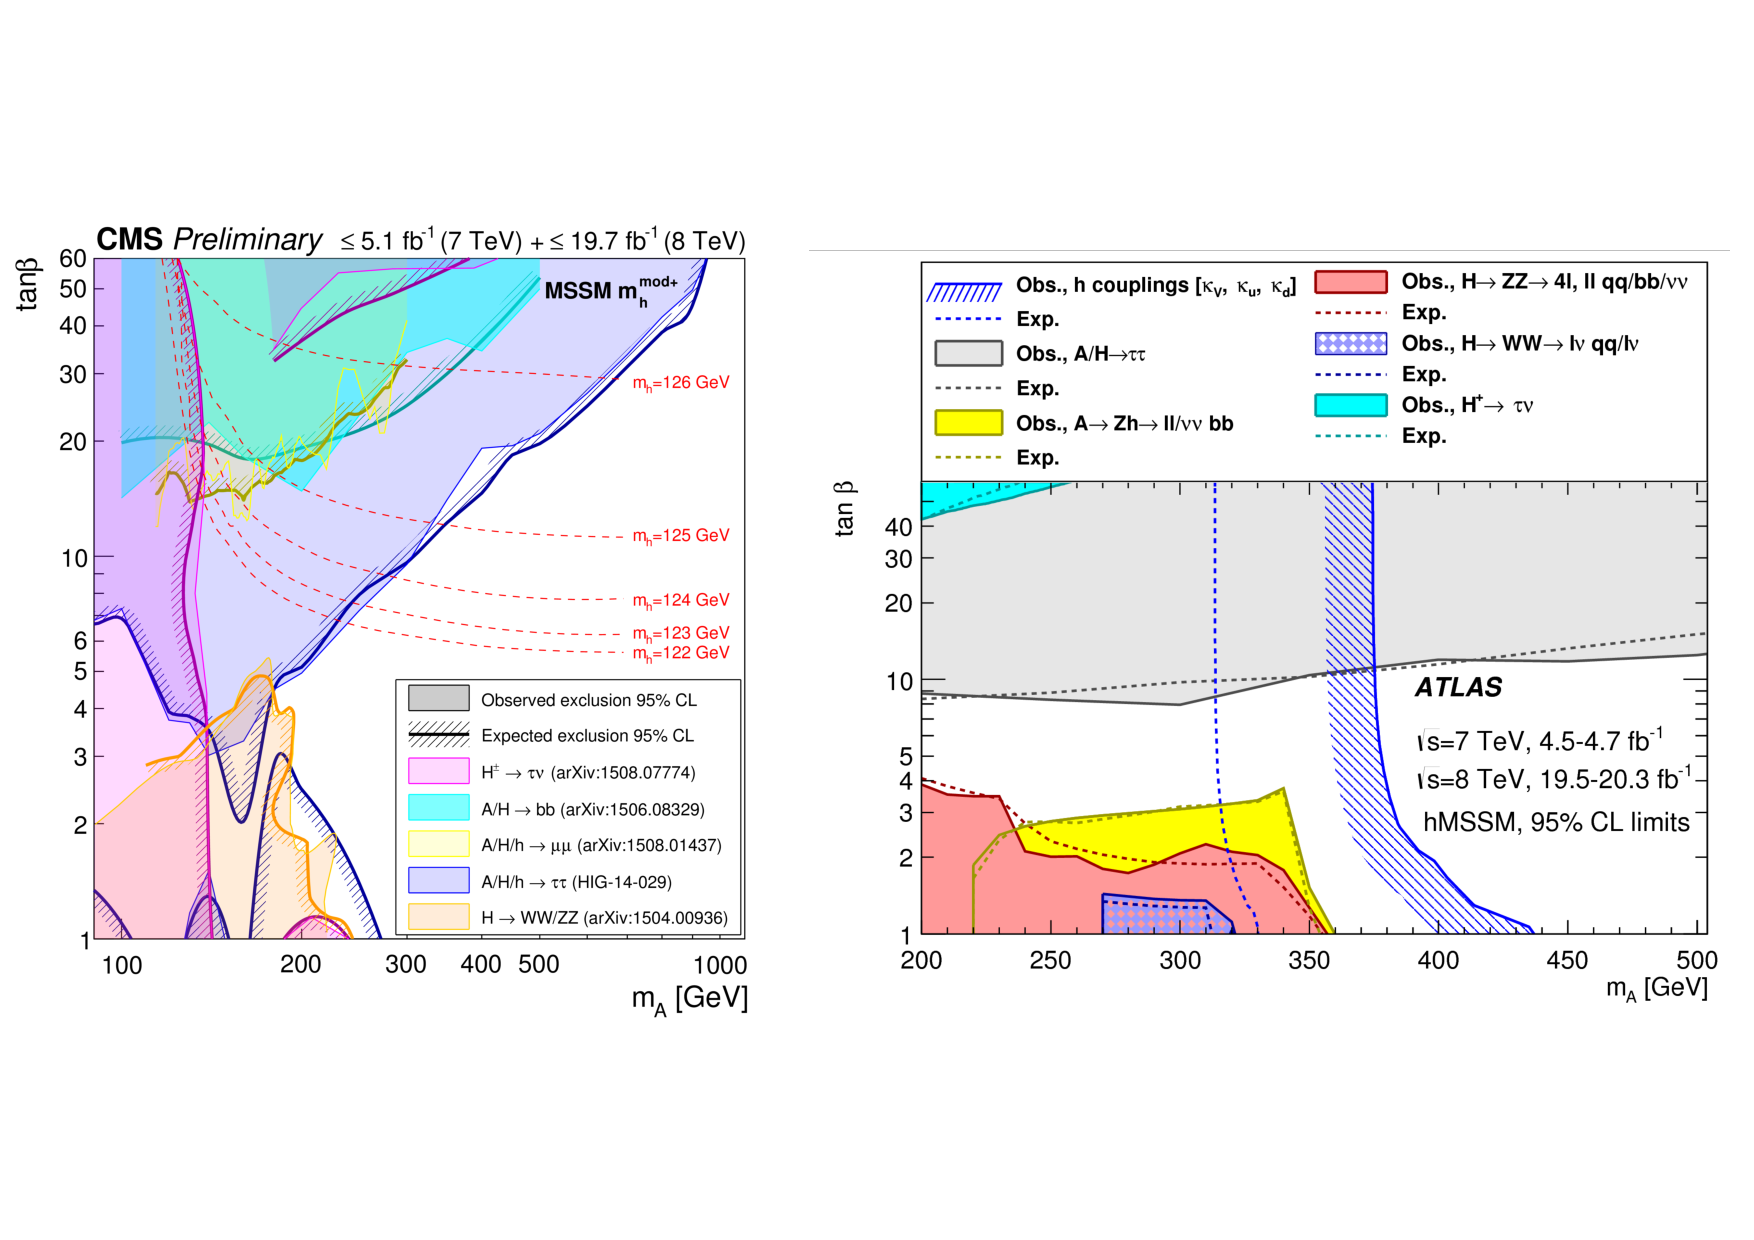
\includegraphics[width=0.9\textwidth, angle=0] {figures/MSSM_Run1.pdf}
\caption{Run1 $m_A - tan\beta$ exclusion plane by (left) CMS experiment and (right) ATLAS experiment.}
\label{fig:MSSM_Run1}   
\end{figure}
%%